%
% Main document
% ===========================================================================
% This is part of the document "Project documentation template".
% Authors: brd3
%

%---------------------------------------------------------------------------
\documentclass[
	a4paper,					% paper format
	10pt,							% fontsize
	twoside,					% double-sided
	openright,				% begin new chapter on right side
	notitlepage,			% use no standard title page
	parskip=half,			% set paragraph skip to half of a line
]{scrreprt}					% KOMA-script report
%---------------------------------------------------------------------------

\raggedbottom
\KOMAoptions{cleardoublepage=plain}			% Add header and footer on blank pages


% Load Standard Packages:
%---------------------------------------------------------------------------
\usepackage[standard-baselineskips]{cmbright}

\usepackage[ngerman]{babel}										% german hyphenation
%\usepackage[latin1]{inputenc}  							% Unix/Linux - load extended character set (ISO 8859-1)
\usepackage[ansinew]{inputenc}  							% Windows - load extended character set (ISO 8859-1)
\usepackage[T1]{fontenc}											% hyphenation of words with �,� and �
\usepackage{textcomp}													% additional symbols
\usepackage{ae}																% better resolution of Type1-Fonts 
\usepackage{fancyhdr}													% simple manipulation of header and footer 
\usepackage{graphicx}                      		% integration of images
\usepackage{float}														% floating objects
\usepackage{caption}													% for captions of figures and tables
\usepackage{booktabs}													% package for nicer tables
\usepackage{tocvsec2}													% provides means of controlling the sectional numbering
%---------------------------------------------------------------------------

% Load Math Packages
%---------------------------------------------------------------------------
\usepackage{amsmath}                    	   	% various features to facilitate writing math formulas
\usepackage{amsthm}                       	 	% enhanced version of latex's newtheorem
\usepackage{amsfonts}                      		% set of miscellaneous TeX fonts that augment the standard CM
\usepackage{amssymb}													% mathematical special characters
\usepackage{exscale}													% mathematical size corresponds to textsize
%---------------------------------------------------------------------------

% Package to facilitate placement of boxes at absolute positions
%---------------------------------------------------------------------------
\usepackage[absolute]{textpos}
\setlength{\TPHorizModule}{1mm}
\setlength{\TPVertModule}{1mm}
%---------------------------------------------------------------------------					
			
% Definition of Colors
%---------------------------------------------------------------------------
\RequirePackage{color}                          % Color (not xcolor!)
\definecolor{linkblue}{rgb}{0,0,0.8}            % Standard
\definecolor{darkblue}{rgb}{0,0.08,0.45}        % Dark blue
\definecolor{brickred}{cmyk}{0,0.89,0.94,0.28}  % Brickred
%\definecolor{linkcolor}{rgb}{0,0,0.8}     			% Blue for the web- and cd-version!
\definecolor{linkcolor}{rgb}{0,0,0}        			% Black for the print-version!
\definecolor{bfhred}{rgb}{0.776,0,0.066}  			% Red
%---------------------------------------------------------------------------

% Hyperref Package (Create links in a pdf)
%---------------------------------------------------------------------------
\usepackage[
	pdftex,ngerman,bookmarks,plainpages=false,pdfpagelabels,
	backref = {false},										% No index backreference
	colorlinks = {true},                  % Color links in a PDF
	hypertexnames = {true},               % no failures "same page(i)"
	bookmarksopen = {true},               % opens the bar on the left side
	bookmarksopenlevel = {0},             % depth of opened bookmarks
	pdftitle = {Projekt 2 - AI Challenge},	   	% PDF-property
	pdfauthor = {kases1 kustl1},        					  % PDF-property
	pdfsubject = {LaTeX Template},        % PDF-property
	linkcolor = {linkcolor},              % Color of Links
	citecolor = {linkcolor},              % Color of Cite-Links
	urlcolor = {linkcolor},               % Color of URLs
]{hyperref}
%---------------------------------------------------------------------------

% Set up page dimension
%---------------------------------------------------------------------------
\usepackage{geometry}
\geometry{
	a4paper,
	left=28mm,
	right=15mm,
	top=30mm,
	headheight=20mm,
	headsep=10mm,
	textheight=242mm,
	footskip=15mm
}
%---------------------------------------------------------------------------

% Makeindex Package
%---------------------------------------------------------------------------
\usepackage{makeidx}                         		% To produce index
\makeindex                                    	% Index-Initialisation
%---------------------------------------------------------------------------

% Glossary Package
%---------------------------------------------------------------------------
% the glossaries package uses makeindex
% if you use TeXnicCenter do the following steps:
%  - Goto "Ausgabeprofile definieren" (ctrl + F7)
%  - Select the profile "LaTeX => PDF"
%  - Add in register "Nachbearbeitung" a new "Postprozessoren" point named Glossar
%  - Select makeindex.exe in the field "Anwendung" ( ..\MiKTeX x.x\miktex\bin\makeindex.exe )
%  - Add this [ -s "%tm.ist" -t "%tm.glg" -o "%tm.gls" "%tm.glo" ] in the field "Argumente"
%
% for futher informations go to http://ewus.de/tipp-1029.html
%---------------------------------------------------------------------------
\usepackage[nonumberlist]{glossaries}
\makeglossaries
\newglossaryentry{Tile}{name={Tile},description={Ortsangabe auf dem Spielfeld mit Row (Zeile) und Column (Spalte) beschrieben. Bsp: <r:12 c:10>}}
\newglossaryentry{FogofWar}{name={Fog of War},description={Teil der Karte, der durch die eigenen Einheiten nicht mehr sichtbar ist}}
\newglossaryentry{AI}{name={AI},description={Artificial Intelligence - K�nstliche Intelligenz}}
\newglossaryentry{Bot}{name={Bot},description={AI-Agent f�r ein Computerspiel}}
\newglossaryentry{API}{name={API},description={Application Programming Interface - Programmierschnittstelle}}
\newglossaryentry{InfluenceMap}{name={Influence Map},description={Datenstruktur, die zur Berechnung des Einflusses von Spieleinheiten auf die Spielkarte dient}}
\newglossaryentry{LazyInitialization}{name={Lazy Initialization},description={Bei der Lazy Initialization wird eine Ressource erst beim erstmaligen Gebrauch initialisiert (z.B. ein Logfile erst mit dem ersten Log-Eintrag erstellt)}}

%---------------------------------------------------------------------------

% Intro:
%---------------------------------------------------------------------------
\begin{document}                              	% Start Document
\settocdepth{section}														% Set depth of toc
\pagenumbering{roman}														
%---------------------------------------------------------------------------

% Set up header and footer
%---------------------------------------------------------------------------
\fancyhf{}																		% clean all fields
\fancypagestyle{plain}{												% new definition of plain style
	\fancyfoot[OR,EL]{\footnotesize \thepage} 	% footer right part --> page number
	\fancyfoot[OL,ER]{\footnotesize \leftmark}	% footer left part -->	chapter
	\fancyhead[C]{															% header center part --> BFH logo
		\begin{textblock}{0}[0,0](86,9)
			
\includegraphics[scale=1.0]{bilder/bfh_de_without_text.pdf}
		\end{textblock}
	}
}

\renewcommand{\chaptermark}[1]{\markboth{\thechapter.  #1}{}}
\renewcommand{\headrulewidth}{0pt}				% no header stripline
\renewcommand{\footrulewidth}{0pt} 				% no bottom stripline

\pagestyle{plain}
%---------------------------------------------------------------------------


% Title Page and Abstract
%---------------------------------------------------------------------------
%
% Project documentation template
% ===========================================================================
% This is part of the document "Project documentation template".
% Authors: brd3
%

\begin{titlepage}


% Red Bar and BFH-Logo absolute placed at (87,10) on A4
% Actually not a realy satisfactory solution but working.
%---------------------------------------------------------------------------
\setlength{\unitlength}{1mm}
\begin{textblock}{210}(-10,-10)
	\begin{picture}(210,32)
		\put(0,0){\color{bfhred}\rule{240mm}{30mm}}
	\end{picture}
\end{textblock}

\begin{textblock}{0}[0,0](84,7)
	
\includegraphics[scale=1.0]{90_bilder/bfh_de_white.pdf}
\end{textblock}

% Titel / Untertitel / Autor:
%---------------------------------------------------------------------------
\begin{flushleft}

\vspace*{4cm}

\fontsize{12pt}{15pt}\selectfont\vspace{0.5em}
Fachbereich Technik und Informatik \\
Herbstsemester 2012

\vspace{2cm}

\fontsize{30pt}{32pt}\selectfont 
\noindent \textbf{Bachelor Thesis - AI Bot f�r Computerspiele} \\
\fontsize{20pt}{22pt}\selectfont 
\noindent \textbf{Ants AI Challenge} \\


\vspace{4cm}
\fontsize{12pt}{15pt}\selectfont
\begin{tabbing}
xxxxxxxxxxxxxxx\=xxxxxxxxxxxxxxxxxxxxxxx \kill
Studierende:	\> Lukas Kuster			\\
							\> Stefan K�ser		\\
																\\
Betreuung:	\> Dr. J�rgen Eckerle	\\
																\\
Experte:	\> Dr. Federico Fl�ckiger	\\
																\\
																\\
Datum:				\> \today					\\
Version:			\> V01.00					\\
\end{tabbing}
\end{flushleft}

%\vspace{6mm}
%\fontsize{12pt}{15pt}\selectfont
%Dieses Dokument dient als Vorlage f�r die Erstellung von Berichten nach den Richtlinien der BFH. Die Vorlage ist in \LaTeX{} %erstellt und unterst�tzt das automatische Erstellen von diversen Verzeichnissen, Literaturangaben, Indexierung und Glossaren. %Dieser kleine Text ist eine Zusammenfassung �ber das vorliegenden Dokument mit einer L�nge von 4 bis 6 Zeilen.

\end{titlepage}

%
% ===========================================================================
% EOF
%

\cleardoubleemptypage
\setcounter{page}{1}
%\chapter*{Management Summary}
\label{chap:managementSummary}

Ants AI Challenge ist ein Programmierwettbewerb, bei welchem ein Bot programmiert wird der ein Ameisenvolk steuert. Das Ameisenvolk soll auf einer Map Futtersuchen sowie gegnerische V�lker angreifen und vernichten. Dabei m�ssen Problem wie die Pfadsuche, das Verteilen von Aufgaben sowie das Schwarmverhalten gel�st werden. In unserer Arbeit wollten wir herausfinden was es alles braucht um einen solchen intelligenten Bot zu schreiben und gegen andere Mitspieler anzutreten. Wir konzetrierten uns auf die Aufgabenverteilung sowie die Pfadsuche. Diese Erfahrungen wollen wir f�r die Bachelorarbeit mitnehmen, wo wir an einer aktiven Challenge teilnehmen m�chten oder uns in der f�r dieses Projekt verwendete Challenge vertiefen.

\vspace{5cm}
\begin{tabbing}
xxxxxxxxxxxxxxxxxxxx\=xxxxxxxxxxxxxxxxxxxxxxx \kill
Datum					\> \today \\ \\ \\
Name Vorname	\> Lukas Kuster \\ \\
Unterschrift	\> ......................................................... \\ \\ \\
Name Vorname	\> Stefan K�ser \\ \\
Unterschrift	\> .........................................................
\end{tabbing}


%---------------------------------------------------------------------------

% Table of contents and listings
%---------------------------------------------------------------------------
%\tableofcontents
%\listoffigures
%\listoftables
%\cleardoublepage
%---------------------------------------------------------------------------

% Main part:
%---------------------------------------------------------------------------
\pagenumbering{arabic}

\chapter{Einleitung}
\label{chap:einleitung}
Nachdem wir uns im Rahmen des Moduls ''Projekt 2`` (7302) mit der Implementierung eines Bots f�r den Online-Wettbewerb Ants AI-Challenge\footnote{\url{http://www.aichallenge.org}} besch�ftigt hatten, haben wir uns f�r die Bachelorarbeit eine Verbesserung dieses Bots vorgenommen. Ziel des Wettbewerbs ist es jeweils, einen Bot zu programmieren, der durch geschickten Einsatz von KI-Technologien das Spiel m�glichst erfolgreich bestreiten kann.

Im ''Projekt 2`` hatten wir zwar einen Bot implementiert, der alle Aspekte des Spiels einigermassen beherrscht, dazu geh�ren Nahrung sammeln, die Gegend entdecken, H�gel erobern und verteidigen, sowie gegen feindliche Ameisen k�mpfen. Einige dieser F�higkeiten waren aber eher rudiment�r ausgebaut, da wir uns vor allem auf die Pfadsuche konzentriert hatten.

In der Bachelorarbeit ging es nun darum, die taktischen und strategischen Fertigkeiten des Bots auszubauen. Der Schwerpunkt lag auch bei der Bachelorarbeit nicht auf der Optimierung einer Teilaufgabe, sondern auf der Implementierung eines ausgewogenen Bots, der alle Aspekte des Spiels gleichermassen gut beherrscht.

Ein besonderes Augenmerk legten wir dabei auf einen modularen Aufbau des Codes. Nebst einem sauberen objektorientierten Programmdesign spiegelt sich das vor allem in den separaten Modulen ''AITools-Api``, ''Search`` und ''Strategy``, die so generisch implementiert wurden, dass sie mit geringem Aufwand auch in anderen Projekten einsetzbar sind.




\newcommand{\vspacecm}{0.7cm}

\chapter{Ziele}

Der im Rahmen von Projekt 2 entwickelte Bot soll um Logik f�r taktische und strategische Entscheidungen und koordinierte Bewegung erweitert werden.

\section{Funktionale Anforderungen}
\label{sec:ziele.FunktionaleAnforderungen}

\subsection{Musskriterien}
\label{sec:ziele.FunktionaleAnforderungen.Musskriterien}

Der Bot unterscheidet zwischen diversen Aufgaben:
	\begin{itemize}
	\item Nahrungsbeschaffung
	\item Angriff
	\item Verteidigung
	\item Erkundung
	\end{itemize}

\vspace{\vspacecm}

Der Bot kann eine Beurteilung seiner Situation auf dem Spielfeld vornehmen
	\begin{itemize}
	\item Dominante/unterlegene Position
	\item Sicherheit verschiedener Gebiete des Spielfelds (eigener/gegnerischer Einfluss)
	\item Konfliktpotenzial in verschiedenen Gebieten des Spielfelds
	\end{itemize}
		
Anhand der Situationsbeurteilung werden die unterschiedlichen Aufgaben entsprechend gewichtet. Stark gewichtete Aufgaben erhalten mehr Ressourcen (Ameisen) zur Durchf�hrung.

\vspace{\vspacecm}

Der Bot identifiziert zur Erf�llung dieser Aufgaben taktische Ziele:
	\begin{itemize}
	\item Gegnerische H�gel angreifen, was bei Erfolg den Score erh�ht und das eigentliche Ziel des Spiels ist.
	\item Isolierte gegnerische Ameisen angreifen.
	\item Schwachstellen in der gegnerischen Verteidigung ausnutzen.
	\item Engp�sse im Terrain sichern bzw. versperren.
	\item Konfliktzonen, d.h. viele Ameisen auf einem engen Raum, erkennen und entsprechend reagieren.
	\end{itemize}

\vspace{\vspacecm}

F�r die konkrete Erreichung dieser definierten Ziele verf�gt der Bot �ber taktische Logik:
	\begin{itemize}
	\item Bei der Pfadsuche wird die Sicherheit der zu durchquerenden Gebiete ber�cksichtigt
	\item In Kampfsituationen kann der Bot die Ameisen in Formationen gliedern, die geeignet sind, eine lokale �berzahl eigener gegen�ber gegnerischen Ameisen zu erzeugen
	\item Beim Aufeinandertreffen mit gegnerischen Ameisen wird Entschieden ob angegriffen, die Stellung gehalten oder gefl�chtet wird.
	\end{itemize}

\subsection{Kannkriterien}
\label{sec:ziele.FunktionaleAnforderungen.Kannkriterien}
Das Verhalten des Bots ist konfigurativ einstellbar, so dass zum Beispiel ein �agressiver� Bot gegen einen defensiven Bot antreten kann.

\section{Nicht funktionale Anforderungen}
\label{sec:ziele.NichtFunktionaleAnforderungen}

\subsection{Musskriterien}
\label{sec:ziele.NichtFunktionaleAnforderungen.Musskriterien}
Modularer Aufbau, so dass die einzelnen Komponenten getestet werden k�nnen.

Wichtige Funktionen wie die Pfadsuche und die Berechnung von Influence Maps sollen in separaten Modulen implementiert werden, damit sie auch von anderen Projekten verwendet werden k�nnten.

Der Code wird dokumentiert, so dass dieser nachvollziehbar ist.

\subsection{Kannkriterien}
\label{sec:ziele.NichtFunktionaleAnforderungen.Kannkriterien}
F�r die wiederverwendbaren Module wird jeweils ein kleines Tutorial geschrieben, wie die Module verwendbar sind.


\section{Abgrenzungskriterien}

TODO
\chapter{Rahmenbedingungen}

\section{Spielbeschrieb}
\label{sec:spielbeschrieb}

\subsection{Der Wettbewerb}
\label{sec:spielbeschrieb_wettbewerb}
Die AI Challenge\footnote{\url{http://www.aichallenge.org}} ist ein internationaler Wettbwerb des University of Waterloo Computer Science Club der im Zeitraum Herbst 2011 bis Januar 2012 zum 3. Mal stattgefunden hat. Das Spiel ist ein zugbasiertes Multiplayerspiel in welchem sich Ameisenv�lker gegenseitig bek�mpfen. Ziel einer AI-Challenge ist es, einen Bot zu schreiben, der die gegebenen Aufgaben mit m�glichst intelligenten Algorithmen l�st. Die zu l�senden Aufgaben der Ants AI Challenge sind die Futtersuche, das Explorieren der Karten, das Angreifen von gegnerischen V�lkern und deren Ameisenhaufen sowie dem Sch�tzen des eigenen Ameisenhaufen.

\subsection{Spielregeln}
\label{sec:spielbeschrieb_spielregeln}
Nachfolgend sind die wichtigsten Regeln, die w�hrend dem Spiel ber�cksichtigt werden m�ssen, aufgelistet.
\begin{itemize} 
\item Pro Zug k�nnen alle Ameisen um ein Feld (vertikal oder horizontal) verschoben werden.
\item Pro Zug steht insgesamt eine Rechenzeit von einer Sekunde zur Verf�gung. Es d�rfen keine Threads erstellt werden.
\item Bewegt sich eine Ameise in die 4er Nachbarschaft eines Futterpixel, wird dieses eingesammelt. Beim n�chsten Zug entsteht bei dem Ameisenh�gel eine neu Ameise.
\item Die Landkarte besteht aus passierbaren Landpixel sowie unpassierbaren Wasserstellen.
\item Ein Gegener wird geschlagen, wenn im Kampfradius der eigenen Ameise mehr eigene Ameise stehen als gegnerische Ameisen im Kampfradius der Ameise die angegriffen wird.
\item Ein Gegner ist ausgeschieden wenn alle seine eigenen Ameisenh�gel vom Gegner vernichtet wurden. Pro verlorenem H�gel gib es einen Punkteabzug. Pro feindlichen H�gel, der zerst�rt wird gibt es zwei Bonuspunkte.
\item Steht nach einer definierbaren Zeit (Anzahl Z�ge) kein Sieger fest, wird der Sieger anhand der Punkte ermittelt. 
\end{itemize}
Die ausf�hrlichen Regeln k�nnen auf der Webseite nachgelesen werden: \url{http://aichallenge.org/specification.php}

\subsection{Schnittstelle}
\label{sec:spielbeschrieb_schnittstelle}
Die Spielschnittstelle ist simpel gehalten. Nach jeder Spielrunde erh�lt der Bot das neue Spielfeld mittels String-InputStream, die Spielz�ge gibt der Bot dem Spielcontroller mittels String-OutputStream bekannt. Unser MyBot leitet von der Basis-Klasse Bot\footnote{Die Klasse ist im Code unter ants.bot.Bot.Java auffindbar } ab. Ein Spielzug wird im folgendem Format in den Output-Stream gelegt:
\newline
\newline
o <Zeile> <Spalte> <Richtung>
\newline
\newline
Beispiel:
\begin{verbatim}
o 4 7 W
\end{verbatim}
Die Ameise wird von der Position Zeile 4 und Spalte 7 nach Westen bewegt.
\newline
Der Spielcontroller ist in Python realisiert, der Bot kann aber in allen g�ngigen Programmiersprachen wie Java, Python, C\#, C++ etc. geschrieben werden.

\section{Verwendete Software}
\label{sec:software}

Als Entwicklungsumgebung wird Eclipse verwendet. Die Programmierung erfolgt in Java. Die Bachelorarbeit baut auf dem Codestand des Projekt 2 auf. Dieser Stand basiert auf dem Java-Starter-Paket, welches wir von der AI-Challenge Homepage herunter luden und weiterentwickelten. Das Starter-Paket beinhaltet alle n�tigen Komponenten um ein Spiel durchzuf�hren und anzuschauen.

\section{Projektorganisation}
\label{sec:einleitung.Projektorganisation}

\subsection{Beteiligte Personen}
\label{sec:einleitung.Projektorganisation.BetroffenePersonen}

\textbf{Studierende:}\\
 Lukas Kuster \textit{kustl1@bfh.ch} \\
 Stefan K�ser \textit{kases1@bfh.ch}
 
\textbf{Betreuung:}\\
Dr. J�rgen Eckerle \textit{juergen.eckerle@bfh.ch}

\textbf{Experte:}\\
Dr. Federico Fl�ckiger	\textit{federico.flueckiger@bluewin.ch}


\subsection{Projektmeetings}
\label{sec:einleitung.Projektorganisation.Projektmeetings}

\begin{itemize}
\item Es fand jeweils ein Treffen mit dem Betreuer alle 1-2 Wochen statt.
\item Ein Treffen mit dem Experten fand am Anfang der Arbeit statt. Ein zweites Meeting wurde von beiden Seiten nicht f�r notwendig erachtet.
\end{itemize}

\subsection{Arbeitsweise}
\label{sec:einleitung.Projektorganisation.Arbeitsweise}

F�r die gemeinsame Arbeit am Projekt hatten wir uns jeweils den Freitag reserviert. An diesen Tagen arbeiteten wir meist mit Pair-Programming und erzielten dabei gute Fortschritte. Die verbleibenden Aufgaben teilten wir uns auf und arbeiteten einzeln daran. Dabei war die Versionskontrolle mit Git ein sehr hilfreiches Tool, um die Arbeiten zu koordinieren.

Wir arbeiteten mit einem zentralen, �ffentlichen Repository auf GitHub (\url{https://github.com/koschder/ants/}). Nebst dem Vorteil einer vereinfachten Zusammenarbeit bietet GitHub auch einige graphische Auswertungen der Aktivit�t in einem Projekt, die Aufschluss �ber den Verlauf unserer Arbeit geben.

\begin{figure}[H]
\centering
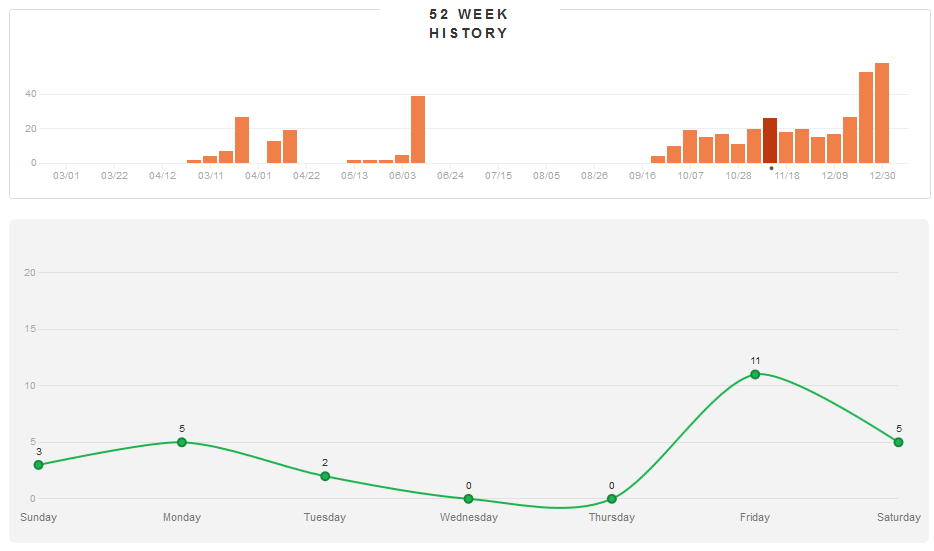
\includegraphics[width=0.99\textwidth]{91_bilder/github/commits}
\caption{Commit History}
\label{fig:commits}
\end{figure}

Die obere H�lfte der Abbildung \ref{fig:commits} zeigt den Aktivit�tsverlauf des Projekts r�ckblickend auf das letzte Jahr. Links, w�hrend den Monaten M�rz, April, Mai und Juni ist der Verlauf des Projekts 2 zu sehen, nach der Sommerpause der Verlauf der Bachelorarbeit. Die Aktivit�tssteigerung gegen Ende des Projekts ist vor allem auf Dokumentations- und Aufr�umarbeiten zur�ckzuf�hren.

Die untere H�lfte zeigt die Anzahl Commits �ber eine Woche verteilt. Man sieht sch�n, dass der Freitag mit Abstand der produktivste Tag war, mit reduzierter Aktivit�t �ber den Rest der Woche verstreut.

\begin{figure}[H]
\centering
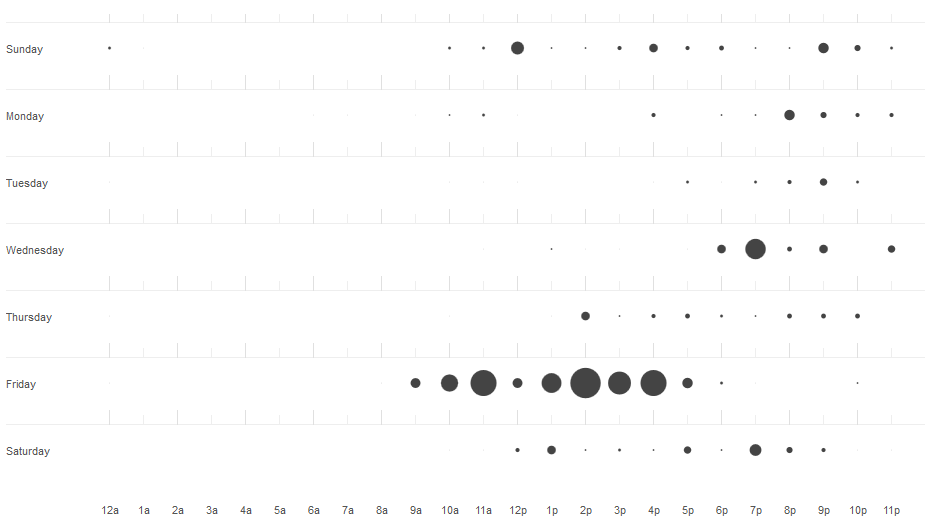
\includegraphics[width=0.99\textwidth]{91_bilder/github/punchcard}
\caption{Aktivit�ten}
\label{fig:punchcard}
\end{figure}

Abbildung \ref{fig:punchcard} zeigt f�r den gesamten Projektverlauf die Zeiten mit der gr�ssten Aktivit�t. Auch hier kann man deutlich erkennen, dass der gr�sste Teil der Arbeit an den Freitagen erstellt wurde.


%\chapter{R�ckblick}
\label{chap:rueckblick}

\section{Resultate}
\label{sec:rueckblick_resultate}
Wir haben mit dieser Arbeit einen guten Einblick in die Programmierung von Bots erhalten. Uns ist bewusst geworden, dass viele Aspekte zusammenspielen m�ssen, damit sich die einzelnen Ameisen intelligent verhalten. Da die Spielschnittstelle einfach gehalten und im Web gut dokumentiert ist kamen wir relativ schnell zu einem sichtbaren Resultat, indem bereits erste Spiele verfolgt werden konnten. Mit einem sauberen Aufbau des Programmcodes konnten wir die Aufgaben einfach gliedern und haben einen guten Grundstein gelegt, falls wir dieses Projekt als Bachelorarbeit weiterverfolgen. Dank den eingesetzten Pfadsuchalgorithmen konnten wir die Rechenzeit verringern und haben so w�hrend einem Zug genug Zeit um weitere Berechnungen zu machen. 

\section{Herausforderungen}
\label{sec:spielbeschrieb_herausforderungen}
Beim Suchen eines Programmierfehlers musste das Logfile durchforstet werden, was sich als eine aufw�ndige und zeitraubende Arbeit herausstellte. Dadurch sind wir auch auf die Idee des Javascript Addon gekommen. Zu Beginn der Arbeit wurde die zur Verf�gung stehende Zeit eines Zuges rasch aufgebraucht, da wir keinen schlauen Algorithmus f�r die Pfadsuche verwendeten; dies konnte mit A* und HPA* behoben werden.

\section{Ziele f�r Bachelorarbeit}
\label{sec:spielbeschrieb_zieleBachelorarbeit}
Im Projekt 2 haben wir uns vor allem auf die Pfadsuche konzentriert. Die Spiele-Entwicklung beinhaltet aber auch Strategie und Taktik. Dies konnte noch nicht angeschaut werden und wird sicher ein Teil der Bachelorarbeit sein. Die Ameisen sollten sich in einem Schwarm fortbewegen, damit sie im Kampf st�rker sind. Dies zu implementieren w�re eine interessante Herausforderung in einem Kerngebiet der K�nstlichen Intelligenz.
Weiter kann gepr�ft werden, ob ein supervised oder ein unsupervised Learning eingebaut werden kann.

Die Organisatoren der AI Challenge sind allerdings bereits dabei, die n�chste Challenge zu planen. Falls sich das n�chste Spiel als geeignet f�r eine Bachelorarbeit erweist, w�rden wir es bevorzugen, an dieser Challenge teilzunehmen, da wir uns so auch direkter mit den anderen Teilnehmern messen k�nnten.


% Attachment:
%---------------------------------------------------------------------------
%\appendix
%\settocdepth{section}
%\chapter{Spielanleitung}
\label{chap:spielanleitung}

\section{Systemvoraussetzungen}
\label{chap:spielanleitung.voraussetzungen}

Um ein Spiel ausf�hren zu k�nnen, muss auf dem Computer folgende Software installiert sein:
\begin{enumerate}
\item Java SE JDK Version 6 \footnote{\url{http://www.oracle.com/technetwork/java/javasebusiness/downloads/java-archive-downloads-javase6-419409.html}}
\item Python \footnote{\url{http://www.python.org/download/}}
\item ANT \footnote{\url{http://ant.apache.org/bindownload.cgi}}
\end{enumerate}

Falls das Spiel mit anderen als den vorkonfigurierten Gegnern gestartet werden soll, muss evtl. noch andere Software installiert werden, je nachdem in welcher Programmiersprache die entsprechenden Bots geschrieben sind.

\section{Ausf�hren eines Spiels}
\label{chap:spielanleitung.Ausfuehrung}
  
Im Ordner \texttt{Code} befinden sich unsere Eclipse-Projekte mit dem gesamten Source-Code unserer Implementation, und der offiziellen Spiel-Engine. Das Hauptprojekt befindet sich im Unterordner \texttt{Ants}. Zum einfachen Ausf\"uhren eines Spiels haben wir dort ein ANT-Buildfile (build.xml) erstellt. Dieses definiert verschiedene Targets, mit denen ein Spiel mit jeweils unterschiedlichen Parametern gestartet werden kann.
Falls ANT korrekt installiert ist, k�nnen diese Targets aus dem \texttt{Ants}-Verzeichnis heraus einfach mit ''\texttt{ant <targetName>}`` aufgerufen werden. 
\begin{enumerate}
\item
Das Target \texttt{testBot} ist lediglich zum einfachen Testen eines Bots sinnvoll und entspricht dem Spiel, das verwendet wird, um Bots, die auf der Website hochgeladen werden, zu testen.
\item
Das Target \texttt{runTutorial} f\"uhrt ein Spiel mit den Parametern aus, die im Tutorial auf der Website zur Erkl\"arung der Spielmechanik verwendet werden.
\item
Die Targets \texttt{mazeAgainst*} f\"uhren jeweils ein Spiel auf einer komplexeren und gr\"osseren, labyrinthartigen Karte aus, und zwar gegen den jeweils bezeichneten Gegner.
\item
Das Target \texttt{maze4Players} f�hrt ein Spiel gegen drei andere Bots auf einer noch etwas gr�sseren Karte durch.
\item
Die Targets \texttt{mazeProfiles} und \texttt{mazeProfiles4Players} sind dazu da, mehrere Kopien unseres Bots mit verschiedenen Profilen gegeneinander antreten zu lassen. Wie im Kapitel \ref{sec:module.Logging.Profile} erw�hnt, muss dazu erst in der Klasse LiveInfo das LiveInfo-Logging deaktiviert werden: 
\lstset{language=Java, tabsize=4}
\begin{lstlisting}
private static boolean enabled = false;
\end{lstlisting}
\item 
Das Target \texttt{testOnline} l�sst den Bot �ber einen privaten TCP-Server gegen andere Bots antreten, unter �hnlichen Bedingungen wie beim eigentlichen Wettbewerb, nur leider mit deutlich weniger Teilnehmern. (s. Kapitel \ref{sec:testCenter.Online})
\item
Die Targets \texttt{repeat*} dienten der Durchf�hrung der Profil-Testl�ufe und sind ansonsten wenig interessant.
\item
Die Targets \texttt{debug*} dienten dem Starten unserer Testbots, die wir w�hrend der Entwicklung einsetzten (s. Kapitel \ref{sec:testCenter.Testbots}).
\end{enumerate}

Bei den meisten dieser Targets erscheint beim Starten eine Abfrage, welches Profil man gerne starten w�rde. Hier stehen die in Kapitel \ref{sec:module.Profile.DefinierteProfile} beschriebenen Profile zur Auswahl.

Im Unterordner \texttt{tools} befindet sich die in Python implementierte Spiel-Engine. Unter \texttt{tools/maps} liegen noch weitere vordefinierte Umgebungen, und unter \texttt{tools/mapgen} liegen verschiedene Map-Generatoren, die zur Erzeugung beliebiger weiterer Karten verwendet werden k\"onnen. 

Im Unterordner \texttt{tools/sample\_bots} befinden sich einige einfache Beispiel-Bots, gegen die man spielen kann. 

Im Unterordner \texttt{tools/bots} haben wir Kopien der Bots von einigen Teilnehmern abgelegt, gegen die wir im Zug der Entwicklung immer wieder getestet haben. 
%\chapter{Weiterer Anhang}
\label{chap:anhang_B}

\section{Test 1}
Phasellus eget velit massa, sed faucibus nisi. Etiam tincidunt libero viverra lorem bibendum ut rutrum nisi volutpat. Donec non quam vitae lacus egestas suscipit at eu nisi. Maecenas non orci risus, at egestas tellus. Vivamus quis est pretium mauris fermentum consectetur. Cras non dolor vitae nulla molestie facilisis. Aliquam euismod nisl eget risus pretium non suscipit nulla feugiat. Nam in tortor sapien. 

\subsection{Umfeld}
Nam lectus nibh, laoreet eu ultrices nec, consequat nec sem. Nulla leo turpis, suscipit in vulputate a, dapibus molestie quam. Vestibulum pretium, purus sed suscipit tempus, turpis purus fermentum diam, id cursus enim mi a tortor. Proin imperdiet varius pellentesque. Nam congue, enim sit amet iaculis venenatis, dui neque ornare purus, laoreet porttitor nunc justo vel velit. Suspendisse potenti. Nulla facilisi.

%---------------------------------------------------------------------------

% Glossary
%---------------------------------------------------------------------------
%\cleardoublepage
%\phantomsection 
%\addcontentsline{toc}{chapter}{Glossar}
%\renewcommand{\glossaryname}{Glossar}
%\printglossary
%---------------------------------------------------------------------------

% Bibliography
%---------------------------------------------------------------------------
%\cleardoublepage
%\phantomsection 
%\addcontentsline{toc}{chapter}{Literaturverzeichnis}
%\bibliographystyle{IEEEtranS}
%\bibliography{datenbanken/bibliography}{}
%---------------------------------------------------------------------------

% Index
%---------------------------------------------------------------------------
%\cleardoublepage
%\phantomsection 
%\addcontentsline{toc}{chapter}{Stichwortverzeichnis}
%\renewcommand{\indexname}{Stichwortverzeichnis}
%\printindex
%---------------------------------------------------------------------------

%---------------------------------------------------------------------------
\end{document}

